\documentclass[pdftex,12pt,a4paper]{article}

\usepackage{graphicx}  
\usepackage[margin=2.5cm]{geometry}
\usepackage{breakcites}
\usepackage{indentfirst}
\usepackage{pgfgantt}
\usepackage{pdflscape}
\usepackage{float}
\usepackage{epsfig}
\usepackage{epstopdf}
\usepackage[cmex10]{amsmath}
\usepackage{stfloats}
\usepackage{multirow}

\renewcommand{\refname}{REFERENCES}
\linespread{1.3}

\usepackage{mathtools}
%\newcommand{\HRule}{\rule{\linewidth}{0.5mm}}
\thispagestyle{empty}
\begin{document}
\begin{titlepage}
\begin{center}
\textbf{}\\
\textbf{\Large{ISTANBUL TECHNICAL UNIVERSITY}}\\
\vspace{0.5cm}
\textbf{\Large{COMPUTER ENGINEERING DEPARTMENT}}\\
\vspace{2cm}
\textbf{\Large{BLG 242E\\ DIGITAL CIRCUITS LABORATORY\\ HOMEWORK 2}}\\
\vspace{2.8cm}
\begin{table}[ht]
\centering
\Large{
\begin{tabular}{lcl}
\textbf{HOMEWORK NO}  & : & 2 \\
\textbf{HOMEWORK DATE}  & : & 7.04.2023\\
\textbf{LAB SESSION}  & : & FRIDAY - 10.30 \\
\textbf{GROUP NO}  & : & G8 \\
\end{tabular}}
\end{table}
\vspace{1cm}
\textbf{\Large{GROUP MEMBERS:}}\\
\begin{table}[ht]
\centering
\Large{
\begin{tabular}{rcl}
150200919  & : & Abdullah Jafar Mansour Shamout \\
150220762  & : & Muhammed Yusuf Mermer  \\
\end{tabular}}
\end{table}
\vspace{2.8cm}
\textbf{\Large{SPRING 2023}}

\end{center}

\end{titlepage}

\thispagestyle{empty}
\addtocontents{toc}{\contentsline {section}{\numberline {}FRONT COVER}{}}
\addtocontents{toc}{\contentsline {section}{\numberline {}CONTENTS}{}}
\setcounter{tocdepth}{4}
\tableofcontents
\clearpage

\setcounter{page}{1}

\section{INTRODUCTION}
In this experiment we implemented SR-Latch, D flip-flop, JK flip-flop using only NAND gates. We used 4 JK flip-flop to make synchronous and asynchronous up counters with 4-bits. In synchronous, we connected all of them to clock signal. However for the asynchronous, we connected one's input to another. In the last part we implemented 16 bit circular left shift register with parallel load.

\section{PRELIMINARY}

\subsection{Question 1)}
flip-flops are sequential logic circuits that are characterized with being bistable. Main reason behind the use of flip-flops is they can store information. To store information, they have loops inside. They will keep their values until the next edge occurs, so it will prevent unexpected asynchronous changes. And you can change inputs for the next cycles easily. One can use the output in the other circuits without giving same signals always.


\subsection{Question 2)}
The difference between Latch and Flip-Flop is about time of the change sensed in the output. In latches output changes whenever the one of the input changes. That is why they are called level triggered. However, it is not simple to say it for Flip-Flops. Beside of the input changes, to see the effect in output of the flip-flops, there should be edges in clock signal (high to low or low to high). With this feature, output of the flip-flops will change only in the next clock cycles. It will prevent instant series of effects in the outputs. So we can say flipflops are edge triggered while latches are level triggered.

\subsection{Question 3)}
The SR latch is a bistable memory element that has two inputs set(S) and reset(R). The structure of the SR latch can be made multiple ways, the way we did it was by taking two NAND gates and connecting each ones output to the others input as a feedback system. That means that one NAND gate will have SET as input and the other NAND gate's output as input, while the other will have RESET as an input and the other NAND gate's output as input. The NAND based SR latch is an active low, that means when we give a 0 to set that means we are setting Q to 1, likewise, when we give 0 to reset we are setting Q to 1. This happens due to the properties of the NAND gate, whenever there is a 0 input the output is forced to be 1 regardless of the other input. This is also the reason why  we can't give input as 0 0, because this results in Q and $\sim$Q having the same value which is invalid. However if we give 1 1, that makes the output fully dependent on the other input which makes a no change in the output, thus the same value is retained.
\subsection{Question 4)}
\begin{table}[H]
\begin{tabular}{|c|c|c|c|}
\hline
S & R & Q & $\sim$Q         \\ \hline
0 & 0 & 1/invalid & 1/invalid    \\ \hline
0 & 1 & 1 & 0                 \\ \hline
1 & 0 & 0 & 1                 \\ \hline
1 & 1 & no change & no change  \\ \hline
\end{tabular}
\end{table}
0 0 input is invalid because Q and $\sim$Q are the same when they should be opposite.
\subsection{Question 5)}
\begin{table}[H]
\begin{tabular}{|c|c|c|c|c|}
\hline
enable & S & R & Q & $\sim$Q         \\ \hline
0 & X & X & no change & no change    \\ \hline
1 & 0 & 0 & no change & no change  \\ \hline
1 & 0 & 1 & 0 & 1                 \\ \hline
1 & 1 & 0 & 1 & 0                 \\ \hline
1 & 1 & 1 & 1/invalid & 1/invalid  \\ \hline
\end{tabular}
\end{table}
1 1 input is invalid because Q and $\sim$Q are the same when they should be opposite.

\subsection{Question 6)}

\begin{table}[H]
\begin{tabular}{|c|c|c|c|}
\hline
clock & D & Q & $\sim$Q         \\ \hline
- & X & no change & no change    \\ \hline
$\uparrow$ & 0 & 0 & 1                 \\ \hline
$\uparrow$ & 1 & 1 & 0                 \\ \hline
\end{tabular}
\end{table}

\subsection{Question 7)}


\begin{table}[H]
\begin{tabular}{|c|c|c|c|}
\hline
clock & J & K & Q                 \\ \hline
--    & X & X & Q0 (no change)    \\ \hline
$\uparrow$     & 0 & 0 & Q0 (no change)    \\ \hline
$\uparrow$     & 0 & 1 & 0                 \\ \hline
$\uparrow$     & 1 & 0 & 1                 \\ \hline
$\uparrow$     & 1 & 1 & $\sim$Q0 (toggle) \\ \hline
\end{tabular}
\end{table}

\section{EXPERIMENT}
\subsection{Part 1}
we can make a Kmap to find the characteristic equation of a SR-latch. As it can be seen in the truth table of the SR-latch in the preliminary section, we can see that if we give 0 0 we get an invalid state for our Q regardless of our previous Q value so we dont care about the output of an invalid input. for 0 1 we get Q as 1 regardless of its previous state, and for 1 0 we get Q as 0 regardless of its previous state, and for 1 1 we get Q meaning the same value as it was. if we plot those values on a kmap we get:
    \begin{figure}[H]
    	\centering
    	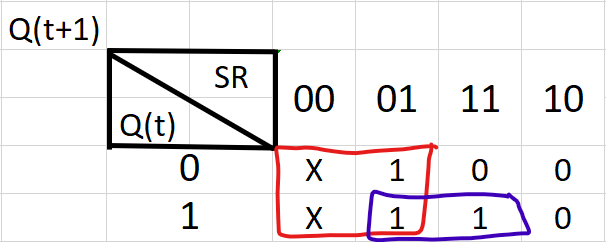
\includegraphics[width=0.8\textwidth]{kmap/sr_char.png}	
    	\caption{SR-latch kmap}
    	\label{SR-latch kmap}
    \end{figure}
from the kmap we realize the characteristic equation will be Q(t+1) = S' + Q(t)R. This is for the NAND gate latch which is an active low, so if we were to give inputs as S' and R' to the latch instead of S and R. we would get the NOR gate characteristic equation which is Q(t+1) = S + Q(t)R'

In the results section we see that when we give 1 1 without any previous inputs we get X X. which is a result of not changing the value of the latch, but since the latch has no presaved value we get this nondeterministic behaviour. And for input 0 0 even though it shows 1 1. this is a forbidden input that should be avoided.
\subsection{Part 2}
we can make a Kmap to find the characteristic equation of the enabled SR-latch. As it can be seen in the truth table of the enabled SR-latch in the preliminary section, we can see that if we give 0 to enabled and any SR or 0 0 to S and R and 1 to enabled we get an no change for our Q regardless of our previous Q value so the output is whatever Q was. For 0 1 to S and R we get Q as 0 regardless of its previous state so we reset it, and for 1 0 we get Q as 1 regardless of its previous state so we set it, and for 1 1 we get an invalid output for Q meaning that we dont care about its output. if we plot those values on a kmap we get:
    \begin{figure}[H]
    	\centering
    	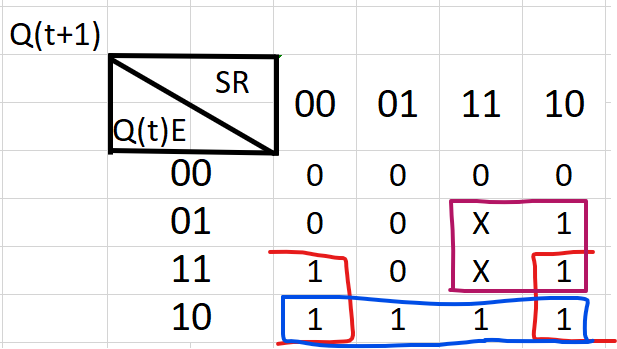
\includegraphics[width=0.8\textwidth]{kmap/enabled_sr.png}	
    	\caption{enabled SR-latch kmap}
    	\label{enabled SR-latch kmap}
    \end{figure}
from the kmap we realize the characteristic equation will be:

Q(t+1) = Q(t)R' + Q(t)E' + SE. 

we can see that this characteristic equation is different than the characteristic equation of a normal NAND SR-latch but same with NOR SR-latch when enable is set to 1 and when enable is set to 0 we get Q(t).

In the results section we see that when we give 0 for enabled or 0 0 to S and R without any previous inputs we get X X. which is a result of not changing the value of the latch, but since the latch has no presaved value we get this nondeterministic behaviour. And for input 1 1 to S and R even though it shows 1 1. this is a forbidden input that should be avoided.
The enabled SR-latch with NAND gate implementation is an active high circuit.

\subsection{Part 3}
We implemented a negative edge triggered D-flipflop from enabled D-latches in this part. To implement it we used a master and slave configuration with an inverted clock to the slave, thus the output would come at NOT clock. The schematics and the simulation van be seen in the results section
\subsection{Part 4}
for the design of a positive edge triggered JK flipflop Using a NAND configured SR flip flop is not possible in structural verilog and would result in a XX state that is why the only other way is to either use behavioral verilog, which we were instructed not to use or use a D flipflop which is what we did. For the implementation of the JK flipflop using a D flipflop we utilized its truthtable and its excitation table to create a conversion table between it and the JK, then we drew its kmap and found this expression D = K'Q + JQnot, then using nand modules we implemented that expression and got our JK-flipflop

\subsection{Part 5}

In the design of asynchronous 4-bit up counter, except the last one, we connected all of the flip-flops to the clock of the next one.


Implementation of this circuit is little bit trickier as to activate all of the flip-flops, we need to initialize them to either to 0 or 1. To do this we need to give J=0 and K=1 or J=1 and K=0. However, giving just insert constant J and K does not help to activate all flip flops as we need waves in outputs to active other flip-flops. For this reason, we gave different, fluctuating values to all the JK flip-flops. We created waves in the outputs to activate consequent flip flops. In here also clock frequency is little bit higher because we wanted to activate all flip-flops very fast.



\begin{table}[H]
\centering
\begin{tabular}{|c|c|c|c|c|}
\hline
\begin{tabular}[c]{@{}c@{}}Clock of the \\ First \\ Flip-Flop\end{tabular} & \begin{tabular}[c]{@{}c@{}}Initial \\ Binary\end{tabular} & \begin{tabular}[c]{@{}c@{}}Initial\\ Decimal\end{tabular} & \begin{tabular}[c]{@{}c@{}}Final\\ Binary\end{tabular} & \begin{tabular}[c]{@{}c@{}}Final\\ Decimal\end{tabular} \\ \hline
$\uparrow$                                                                 & 0000                                                      & 0                                                         & 0001                                                   & 1                                                       \\ \hline
$\uparrow$                                                                 & 0001                                                      & 1                                                         & 0010                                                   & 2                                                       \\ \hline
$\uparrow$                                                                 & 0010                                                      & 2                                                         & 0011                                                   & 3                                                       \\ \hline
$\uparrow$                                                                 & 0011                                                      & 3                                                         & 0100                                                   & 4                                                       \\ \hline
$\uparrow$                                                                 & 0100                                                      & 4                                                         & 0101                                                   & 5                                                       \\ \hline
$\uparrow$                                                                 & 0101                                                      & 5                                                         & 0110                                                   & 6                                                       \\ \hline
$\uparrow$                                                                 & 0110                                                      & 6                                                         & 0111                                                   & 7                                                       \\ \hline
$\uparrow$                                                                 & 0111                                                      & 7                                                         & 1000                                                   & 8                                                       \\ \hline
$\uparrow$                                                                 & 1000                                                      & 8                                                         & 1001                                                   & 9                                                       \\ \hline
$\uparrow$                                                                 & 1001                                                      & 9                                                         & 1010                                                   & 10                                                      \\ \hline
$\uparrow$                                                                 & 1010                                                      & 10                                                        & 1011                                                   & 11                                                      \\ \hline
$\uparrow$                                                                 & 1011                                                      & 11                                                        & 1100                                                   & 12                                                      \\ \hline
$\uparrow$                                                                 & 1100                                                      & 12                                                        & 1101                                                   & 13                                                      \\ \hline
$\uparrow$                                                                 & 1101                                                      & 13                                                        & 1110                                                   & 14                                                      \\ \hline
$\uparrow$                                                                 & 1110                                                      & 14                                                        & 1111                                                   & 15                                                      \\ \hline
$\uparrow$                                                                 & 1111                                                      & 15                                                        & 0000                                                   & 0                                                       \\ \hline
\end{tabular}
\caption{Truth Table of Asynchronous Up Counter }
\label{tab:my-table}
\end{table}


\subsection{Part 6}
Synchronous up counter is relatively easier compered to asynchronous up counter.
We directly connected all clock's inputs to the same pulse, therefore we can activate all flip-flops with giving same JK values. But JK values also depend on the outputs of the former flip-flops. So in order to combine them, we used or gate. We used or gate because we want to assert K values to be 1 at the initial state to activate all of the flip flop with 0 outputs. Then we gave 0 for J and K values except the LSB to not interfere the process. In LSB flip-flop as inputs we gave J=1 and K=1  we need a toggling in the first flip flop. If output of all former flip-flops are 1 then current flip-flop's value will be toggled. With this implementation we successfully made synchronous up counter. 


\begin{table}[H]
\centering
\begin{tabular}{|c|c|c|c|c|}
\hline
\begin{tabular}[c]{@{}c@{}}Clock\\ (same for all)\end{tabular} & \begin{tabular}[c]{@{}c@{}}Initial \\ Binary\end{tabular} & \begin{tabular}[c]{@{}c@{}}Initial\\ Decimal\end{tabular} & \begin{tabular}[c]{@{}c@{}}Final\\ Binary\end{tabular} & \begin{tabular}[c]{@{}c@{}}Final\\ Decimal\end{tabular} \\ \hline
$\uparrow$                                                     & 0000                                                      & 0                                                         & 0001                                                   & 1                                                       \\ \hline
$\uparrow$                                                     & 0001                                                      & 1                                                         & 0010                                                   & 2                                                       \\ \hline
$\uparrow$                                                     & 0010                                                      & 2                                                         & 0011                                                   & 3                                                       \\ \hline
$\uparrow$                                                     & 0011                                                      & 3                                                         & 0100                                                   & 4                                                       \\ \hline
$\uparrow$                                                     & 0100                                                      & 4                                                         & 0101                                                   & 5                                                       \\ \hline
$\uparrow$                                                     & 0101                                                      & 5                                                         & 0110                                                   & 6                                                       \\ \hline
$\uparrow$                                                     & 0110                                                      & 6                                                         & 0111                                                   & 7                                                       \\ \hline
$\uparrow$                                                     & 0111                                                      & 7                                                         & 1000                                                   & 8                                                       \\ \hline
$\uparrow$                                                     & 1000                                                      & 8                                                         & 1001                                                   & 9                                                       \\ \hline
$\uparrow$                                                     & 1001                                                      & 9                                                         & 1010                                                   & 10                                                      \\ \hline
$\uparrow$                                                     & 1010                                                      & 10                                                        & 1011                                                   & 11                                                      \\ \hline
$\uparrow$                                                     & 1011                                                      & 11                                                        & 1100                                                   & 12                                                      \\ \hline
$\uparrow$                                                     & 1100                                                      & 12                                                        & 1101                                                   & 13                                                      \\ \hline
$\uparrow$                                                     & 1101                                                      & 13                                                        & 1110                                                   & 14                                                      \\ \hline
$\uparrow$                                                     & 1110                                                      & 14                                                        & 1111                                                   & 15                                                      \\ \hline
$\uparrow$                                                     & 1111                                                      & 15                                                        & 0000                                                   & 0                                                       \\ \hline
\end{tabular}
\caption{Truth Table of Synchronous Up Counter}
\label{tab:my-table}
\end{table}


\subsection{Part 7}
In positive edge triggering pulse generator, for each bit we used 2 AND gates 1 OR gates. We used AND gates because if load value is given shifting will not work but loading will work. We ORed result of the both and gates. Then when load flag turns back to 0, our design starts to do shifting. In here direct on shift operations are to the left, so that output of the circuit will be the MSB which is turned back to the LSB, later. 



To obtain variable pulse frequencies and duration, we load new values to the system at different test benches. 

For instance to get 1/2 frequency of clock we need to make sequence as 101010... because at every positive edge (which is one cycle of the clock), our pulse generator will return from one to zero or zero to one, which is half cycle because we don't return to the initial state. Clock frequency's 1/4 can be made by doubling consistency of a state like 110011, so this means that two clock cycle needed to convert 1 to 0 and 0 to 1.  

Pulse gap duration rate is little bit different. Sequence of time spent for 0's and 1's are not the same. For 1/7 pulse gap we will spent 1 time for value 1 and 7 for 0. 10000000.....







\section{RESULTS}
\subsection{Schematics and Simulations}

\subsubsection{PART 1}
    \begin{figure}[H]
    	\centering
    	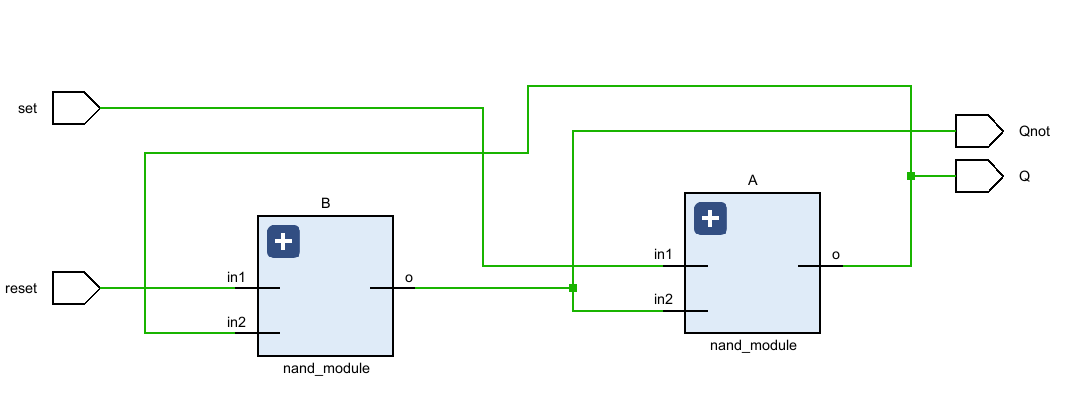
\includegraphics[width=0.8\textwidth]{schematic/sr_schem.png}	
    	\caption{SR-latch schematic}
    	\label{SR-latch schematic}
    \end{figure}
    
    \begin{figure}[H]
    	\centering
    	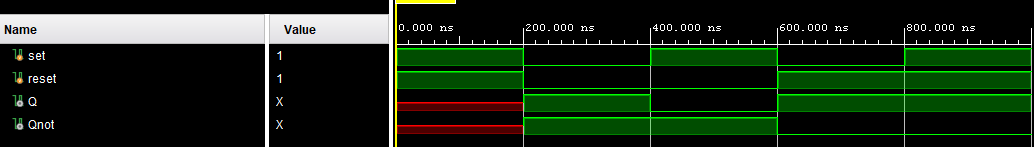
\includegraphics[width=1\textwidth]{simulations/sr_sim.png}	
    	\caption{SR-latch simulation}
    	\label{SR-latch simulation}
    \end{figure}
    
\subsubsection{PART 2}
\begin{figure}[H]
    	\centering
    	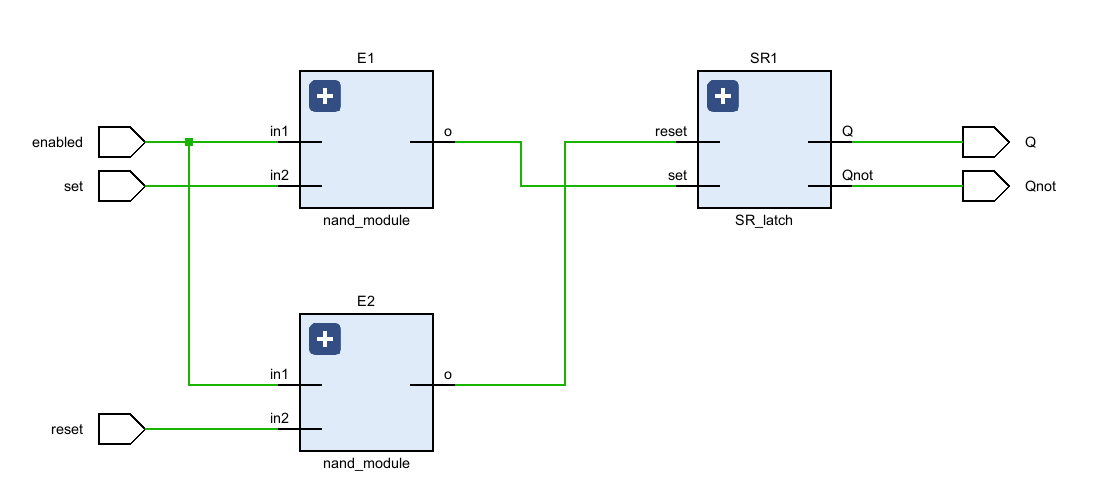
\includegraphics[width=0.8\textwidth]{schematic/enabled_sr.png}	
    	\caption{enabled SR-latch schematic}
    	\label{enabled SR-latch schematic}
    \end{figure}
    
    \begin{figure}[H]
    	\centering
    	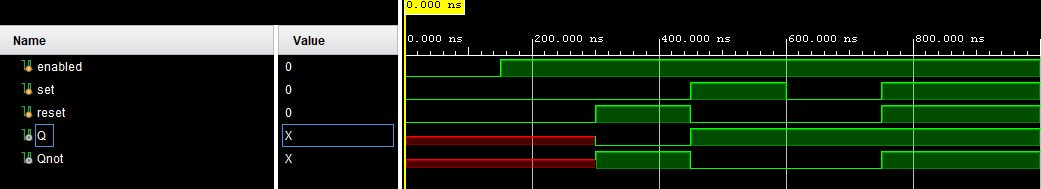
\includegraphics[width=1\textwidth]{simulations/enabled_sr_sim.png}	
    	\caption{enabled SR-latch simulation}
    	\label{enabled SR-latch simulation}
    \end{figure}

\subsubsection{PART 3}
\begin{figure}[H]
    	\centering
    	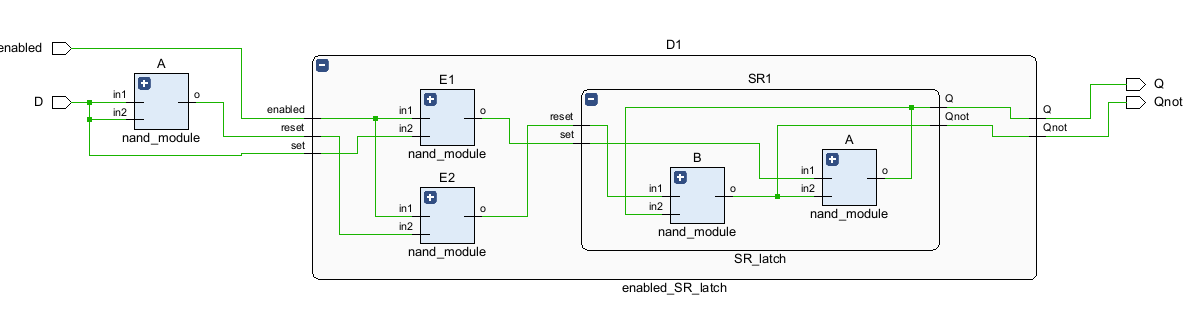
\includegraphics[width=0.8\textwidth]{schematic/D_latch_schem.png}	
    	\caption{enabled D-latch schematic}
    	\label{enabled D-latch schematic}
    \end{figure}
    
\begin{figure}[H]
    	\centering
    	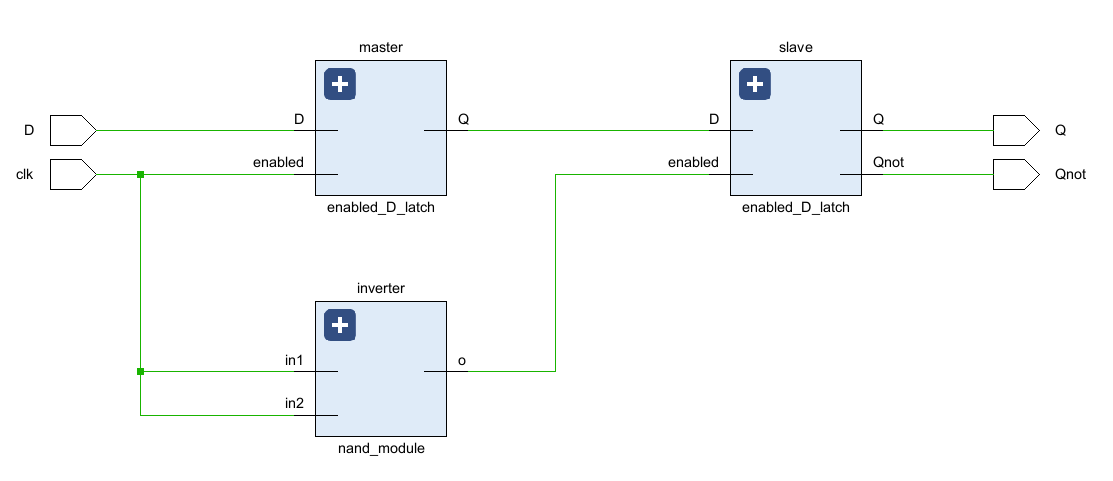
\includegraphics[width=0.8\textwidth]{schematic/D_flip_schem.png}	
    	\caption{D-flip-flop schematic}
    	\label{D-flip-flop schematic}
    \end{figure}
    
    \begin{figure}[H]
    	\centering
    	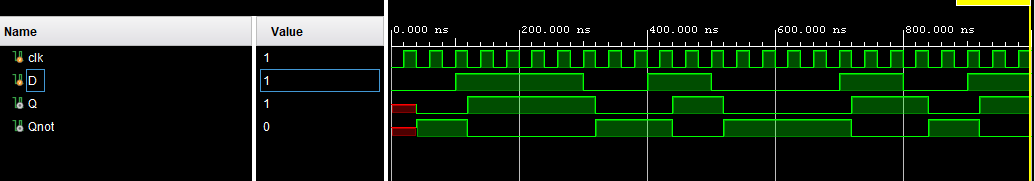
\includegraphics[width=1\textwidth]{simulations/D_sim.png}	
    	\caption{D-flip-flop simulation}
    	\label{D-flip-flop simulation}
    \end{figure}

\subsubsection{PART 4}

\begin{figure}[H]
    	\centering
    	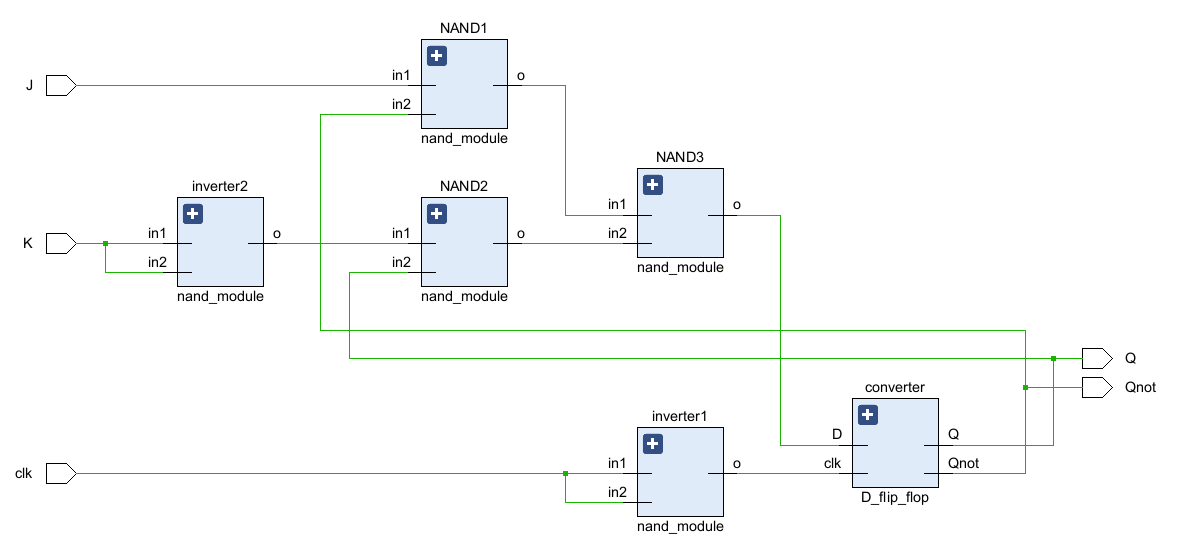
\includegraphics[width=0.8\textwidth]{schematic/JK_schem.png}	
    	\caption{JK-flip-flop schematic}
    	\label{JK-flip-flop schematic}
    \end{figure}
    
    \begin{figure}[H]
    	\centering
    	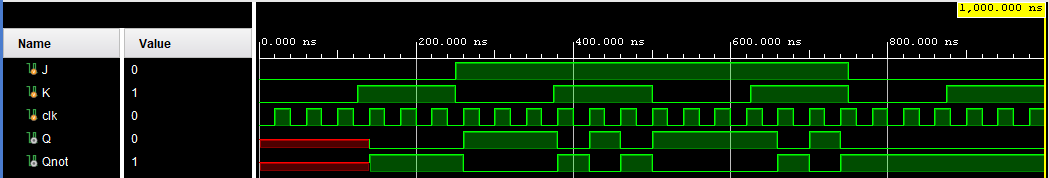
\includegraphics[width=1\textwidth]{simulations/JK_sim.png}	
    	\caption{JK-flip-flop simulation}
    	\label{JK-flip-flop simulation}
    \end{figure}


\subsubsection{PART 5}

\begin{figure}[H]
    	\centering
    	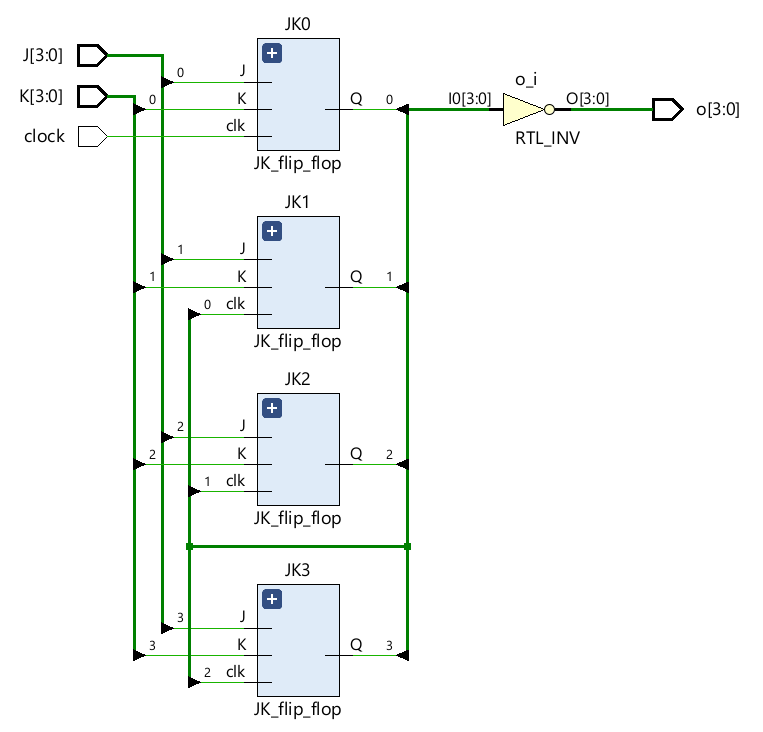
\includegraphics[width=0.8\textwidth]{schematic/async.png}	
    	\caption{Asynchronous Up Counter}
    	\label{Asynchronous Up Counter}
    \end{figure}
    
    \begin{figure}[H]
    	\centering
    	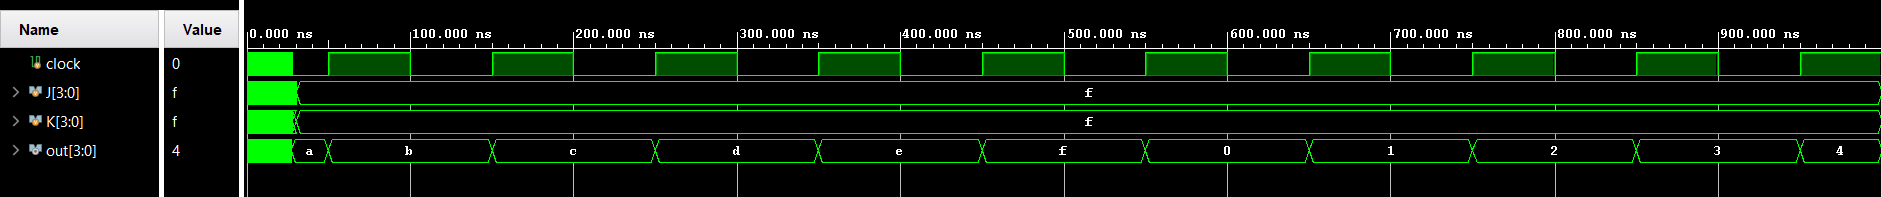
\includegraphics[width=1\textwidth]{simulations/async_sim.png}	
    	\caption{Asynchronous Up Counter simulation}
    	\label{Asynchronous Up Counter}
    \end{figure}




\subsubsection{PART 6}


\begin{figure}[H]
    	\centering
    	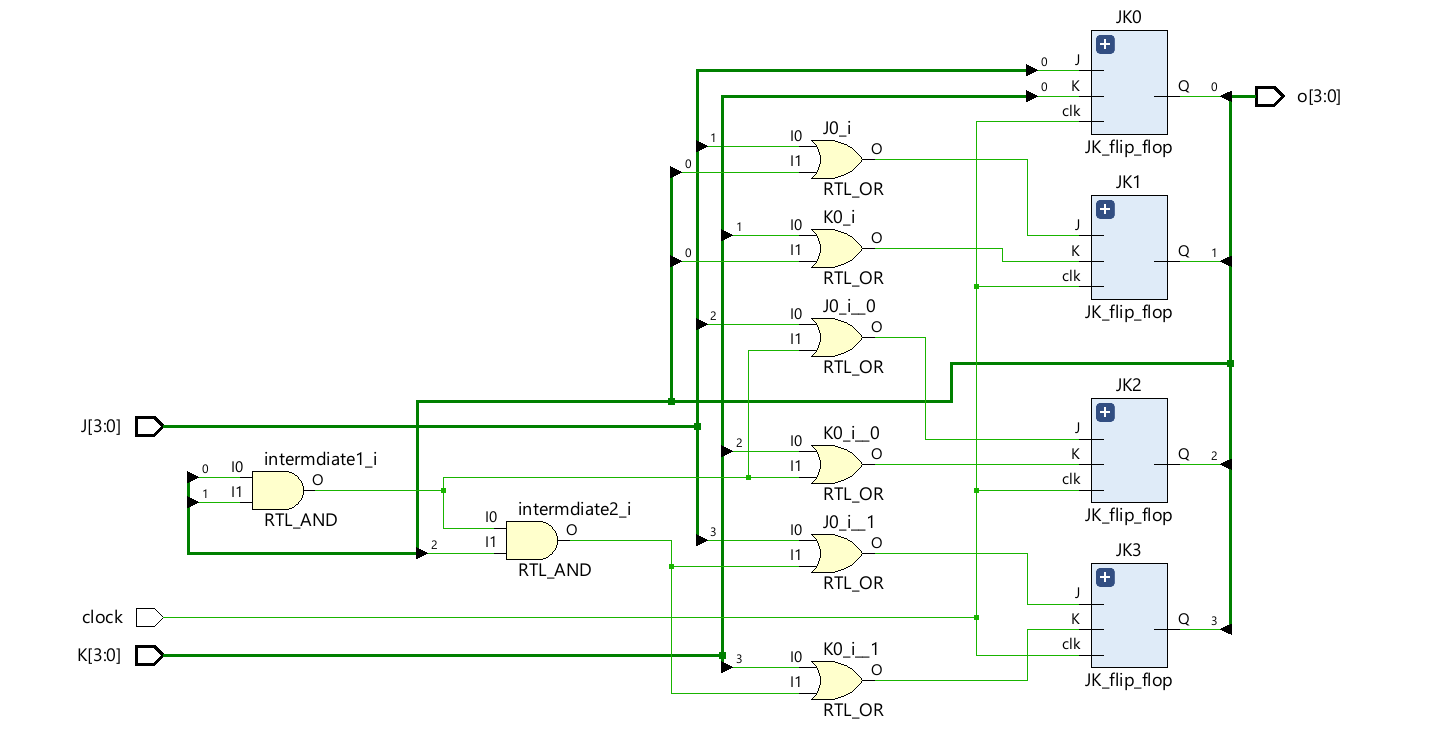
\includegraphics[width=0.8\textwidth]{schematic/sync.png}	
    	\caption{Synchronous Up Counter}
    	\label{Synchronous Up Counter}
    \end{figure}
    
    \begin{figure}[H]
    	\centering
    	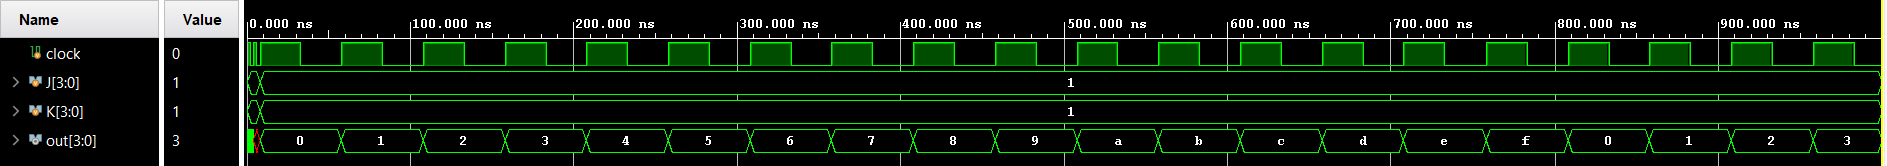
\includegraphics[width=1\textwidth]{simulations/sync_sim.png}	
    	\caption{Synchronous Up Counter simulation}
    	\label{Synchronous Up Counter}
    \end{figure}




\subsubsection{PART 7}

\begin{figure}[H]
    	\centering
    	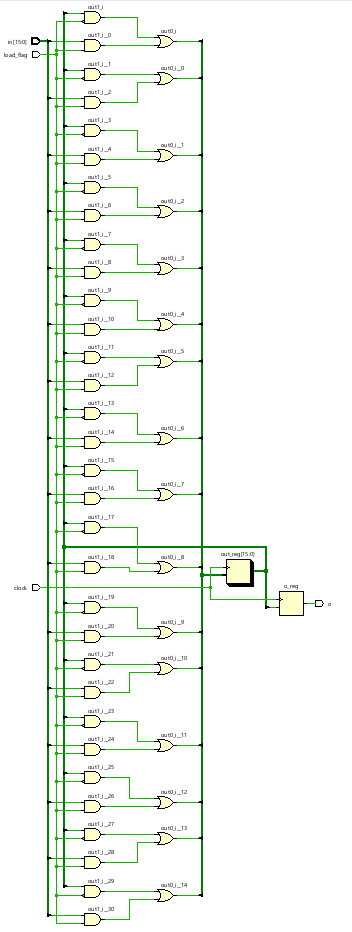
\includegraphics[width=0.4\textwidth]{schematic/pulse.png}	
    	\caption{Positive Edge Triggered Pulse Generator}
    	\label{D-flip-flop schematic}
    \end{figure}
    
    \begin{figure}[H]
    	\centering
    	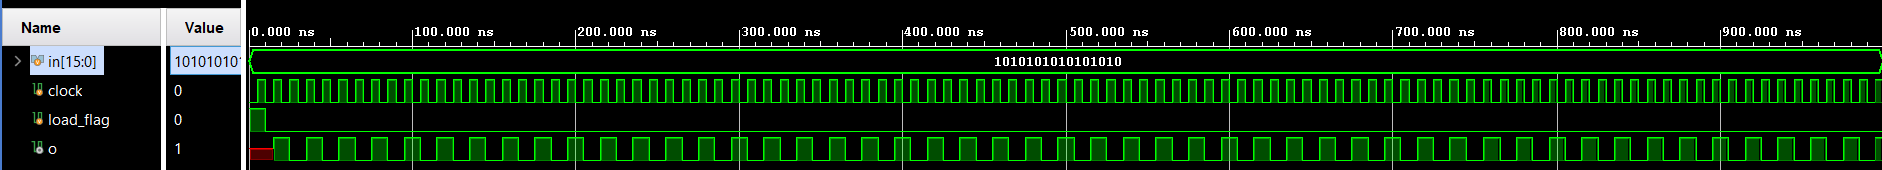
\includegraphics[width=1\textwidth]{simulations/pulse_1_2_freq.png}	
    	\caption{Positive Edge Triggered Pulse Generator with 1/2 frequency of clock}
    	\label{Positive Edge Triggered Pulse Generator}
    \end{figure}


    \begin{figure}[H]
    	\centering
    	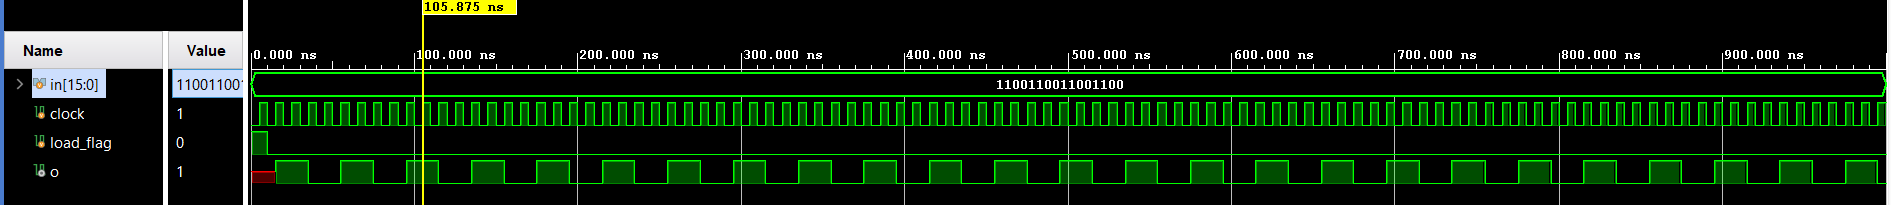
\includegraphics[width=1\textwidth]{simulations/pulse_1_4_freq.png}	
    	\caption{Positive Edge Triggered Pulse Generator with 1/4 frequency of clock}
    	\label{Positive Edge Triggered Pulse Generator}
    \end{figure}


    \begin{figure}[H]
    	\centering
    	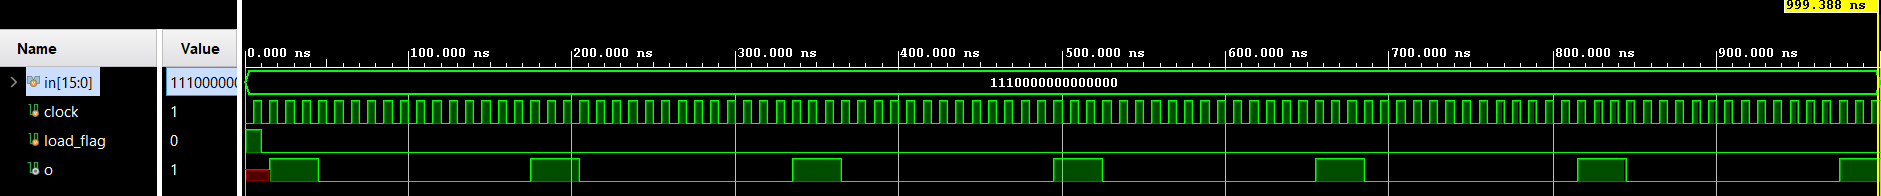
\includegraphics[width=1\textwidth]{simulations/pulse_3_13_gap.png}	
    	\caption{Positive Edge Triggered Pulse Generator with 3/13 pulse gap duration rate}
    	\label{Positive Edge Triggered Pulse Generator}
    \end{figure}

\pagebreak

\section{CONCLUSION}
In this homework, we learned to implement basic latches and flip-flops using NAND gates. Such as SR latch, SR latch with enabled, enabled D-latch, D-flip-flop, JK flip-flop. We had struggle in at first SR flip-flop's as S=1 and R=1 condition have to be avoided. Then especially in JK flip-flop we tried lots and lots of combinations of NAND gates to obtain correct results. However also by discussion with other groups, we come to a result that JK flip-flops cannot be implemented by SR flip-flop made from NAND gates. Therefore, we designed it with D flip-flop instead. Truth table that obtained after simulations are satisfied our expectation.

Then we designed asynchronous and synchronous up counters. For asynchronous, in the test case we gave initial values intentionally to activate all flip-flops properly. In the synchronous we give initial inputs to J's and K's of flip flop's. At the end we got all result like we want from the design.

At the very end question, we designed pulse generator. In here as we can use always block in our module, implementation of the last question was easier. However we had struggle at test bench as we did not get how we can obtain frequencies and gap durations. We thought that it is about differentiation in the clock of pulse generator. Then we found that it is about changes in input load, then we changed our test bench and gave loadFlag=1 just for a small period of time. Then we saw that the pulse generator gives sequential and correct pulses in the simulation. We made our clarifications and saw that our results were correct.
\end{document}

